\documentclass[11pt]{article}
\usepackage{geometry}
\usepackage{enumitem}
\usepackage{graphicx}
\usepackage{hyperref}
\usepackage[usenames,dvipsnames]{color}
\usepackage{caption}
\usepackage{subcaption}
\usepackage{listings}


\renewcommand{\topfraction}{.85}
\renewcommand{\bottomfraction}{.7}
\renewcommand{\textfraction}{.15}
\renewcommand{\floatpagefraction}{.66}
\renewcommand{\dbltopfraction}{.66}
\renewcommand{\dblfloatpagefraction}{.66}
\setcounter{topnumber}{9}
\setcounter{bottomnumber}{9}
\setcounter{totalnumber}{20}
\setcounter{dbltopnumber}{9}
%
\def\MakeMeBlue#1{\textcolor{Blue}{#1}}
\pagenumbering{arabic}
%

\parindent 0pt

%

\title{\MakeMeBlue{The colour preferences in Online Retail Store}}
\author{Uchralt Temuulen}
\date{2018 07 12}

% ========================================================
\begin{document}
\maketitle

% ========================================================
\section{Introduction}

With this project we want to explore the colour preferences in Online Retail. 
In the Information age where people buy online everything, we can get much data about their sales that would help the psychological science. The preferences like which colour is picked most and which combination is most popular.
Also, we try to find groups of the customers and find their similarities and differences. If there were different classes of Customers that behave differently that would impact selling strategies and psychological research. 
For our task we used linear regression model to classify the customers and market basket analyse to search for their retail behaviour on colour combination. 
We found the most frequently bought item colours and also the colour associations to it.
\\


% ========================================================
\section{Related Work}
The work "What we know about Consumer colour Choices"~\cite{a} of Grosman indicates that the products colour play important role in consumers purchase decision.
The paper says that with the knowledge of the costumer colour preferences we can improve the products offering, reduce manufacturing costs and predict new trends immerged in which the marketers feel. It also allows the consumer to make fashion statements which improve the quality of the product. High involvement in product can influence the colour combination in survival but can it also influence in a online gift store?  


The work of Stephen E. Palmera and Karen B. Schlossb   "Color Preference"\cite{b} tell us that certain colour combinations are more preferred than others. Also, it discusses "why they like them." The context is really important. In our case the company sell gifts that means the colour combination indicates positive feeling.    


\newpage
% ========================================================
\section{Methodology}

This Project is done in R Language, which is used often as statistical tool to analyse Data. R has a lot library which is used to clean, analyse and plot the data.\\

 {\large \textbf{1. Get the Data}}\\
We got a massif Set [Data](https://archive.ics.uci.edu/ml/datasets/Online+Retail) of Information which contains all the transactions occurring between 1/12/2010 and 09/12/2011 for a UK-based and registered non-store online retail.The company mainly sells unique all-occasion gifts.
\\
 {\large \textbf{ 2. Inspect the Data Informatio}}n \\
After we imported the data set we checked the information attributes and the quality of the data.

 \textbf{Attributes:} \\
1. InvoiceNo:    Invoice number. Uniquely assigned to each                 transaction. 
                 If this code starts with letter 'c', it  indicates a cancellation. \\
2. StockCode:    Product (item) code. Nominal, a 5-digit integral number uniquely assigned to each distinct product.\\ 
3. Description:  Product (item) name. Nominal. \\
4. Quantity:     The quantities of each product (item) per transaction. Numeric.	\\
5. InvoiceDate:  Invice Date and time. Numeric, the day and time when each transaction was generated. \\
6. UnitPrice:    Unit price. Numeric, Product price per unit in sterling. \\
7. CustomerID:   Customer number. Nominal, a 5-digit integral number uniquely assigned to each customer. \\
8. Country:      Country name. Nominal, the name of the country where each customer resides.\\


\textbf{Quality of the data}
\\
To get the overview of the data we use the summary function from R. In the overview ge get to see how much data is there missing and how are they distributed.  \\


\begin{figure}[!htp]        
  \centering
    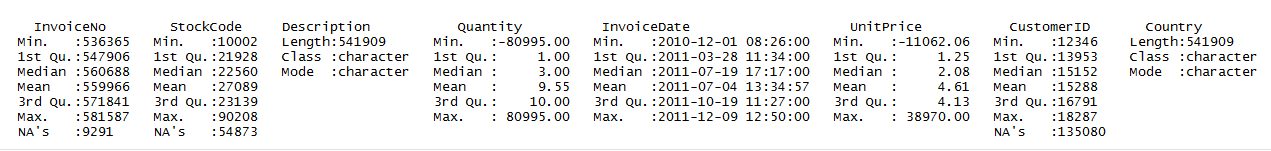
\includegraphics[width=1\textwidth]{pics/summary.jpg}
    \caption{Summary of the Data}
\end{figure}

{\large \textbf{Check the quality of each column in the data clean it accordingly.} }

5. InvoiceNo:    Has low missing values that we can delete. But the cancelation is integrated. Additionaly we must get the Cancelation out and ad it to a additional Column. \\      
6. UnitPrice:    Unitprice has its outliers and negative prices that is unrealistic. We removed the Outliers with filter function because they                are mistakes.\\  
7. Quantity:     Quantity has its obvious Outliers and mistakes like -809995 and 80995 which is also mistakes.  \\                
8. CustomerID:   Has lots of Missing data. We need to replace it with generated numbers with the help of Invoicenumber. \\ 
				 Each Invoicenumber has only one CustomerID\\


{\large\textbf{Get the overall check on the customer behaviour}} \\
First we have to check for some overall behavioural data like overall buying time.
Then we check if there are some correlations between different behaviour and margin.
We had to restructure the data so that we get the new overall information of each customer behaviour with group* and summarize* function. \\


\textbf{Check The Buying Time}

It is important to know when the customer buys. In the daylight or in the evening. The timing can impact the decision of colour.
\begin{figure}[!htp]        
  \centering
    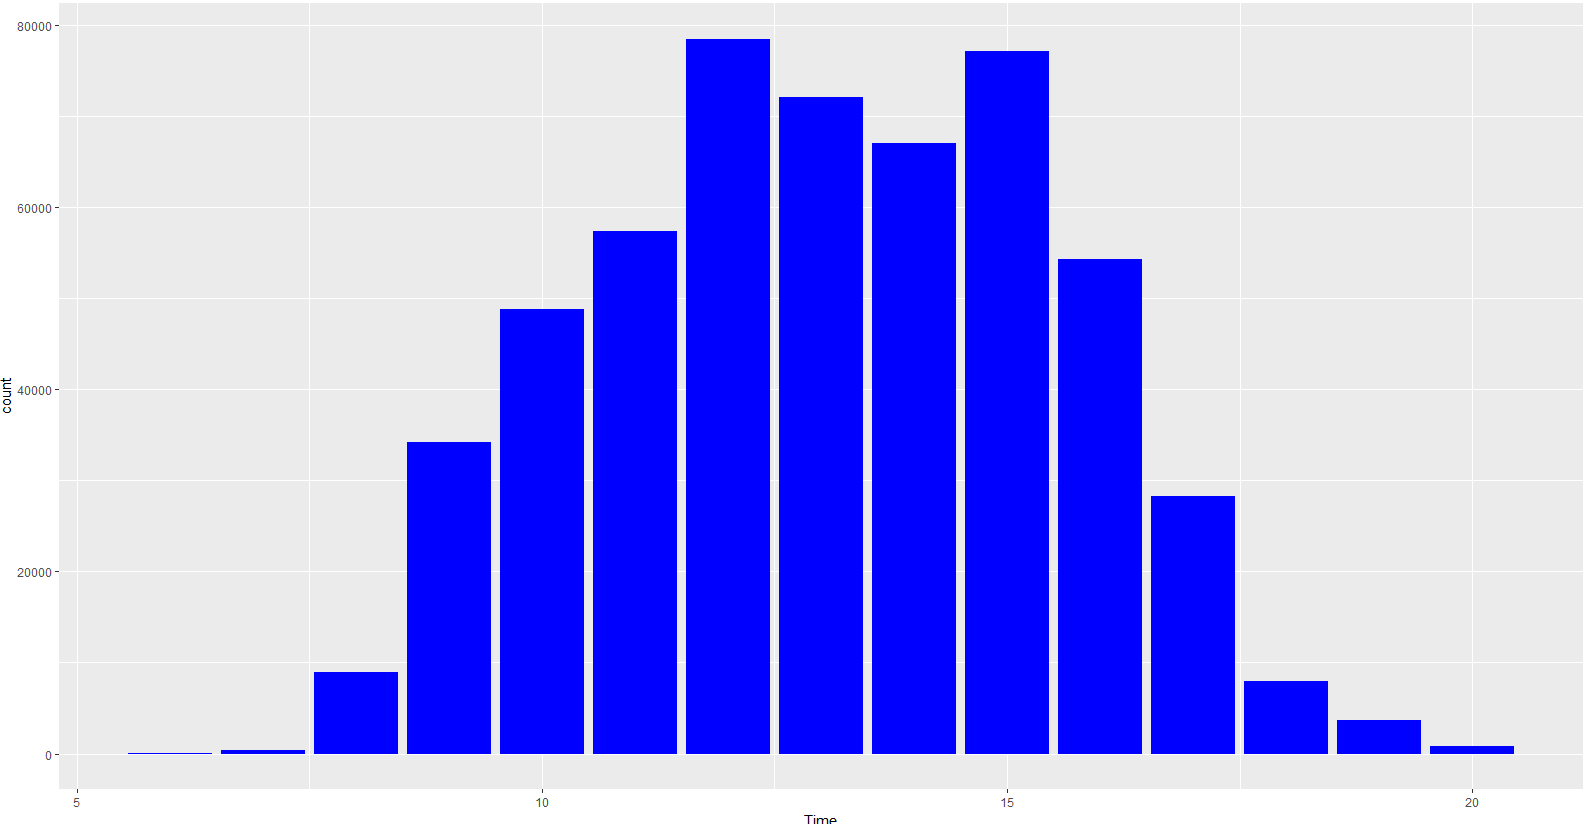
\includegraphics[width=0.7\textwidth]{pics/timebuy.jpg}
    \caption{Buying time.}
\end{figure}

The most buying time is midday that means in daylight and also indicates a working environment?  


\textbf{Check the correlation matrix}\\
It is helpful to know which variable is important for the margin.

\begin{figure}[!htp]        
  \centering
    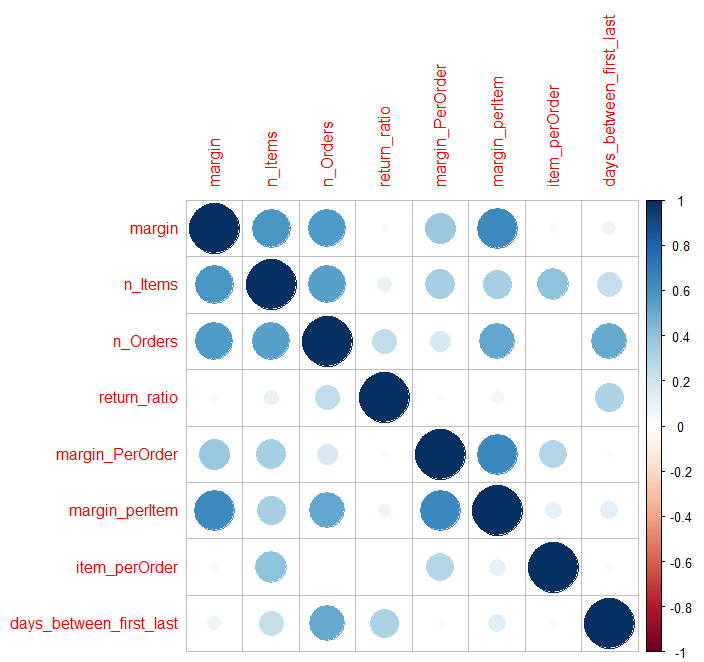
\includegraphics[width=0.4\textwidth]{pics/Korrelation.jpg}
    \caption{Correlation Matrix.}
\end{figure}
margin: how much money each Customer spend whole. \\
nItems: Number of Items each Customer bought. \\
daysbetweenfirstlast: Long time Customer.\\


The Correlation matrix does show us how each behaviour correlates. Customers who buy expensive products do give a lot of margins.\\
Through this correlation matrix we have an idea how to group.\\
\\
\textbf{Check the Customer buying behaviour}\\
To get an idea how to cluster, we are checking the overall margin per count. 


\begin{figure}[!htp]        
  \centering
    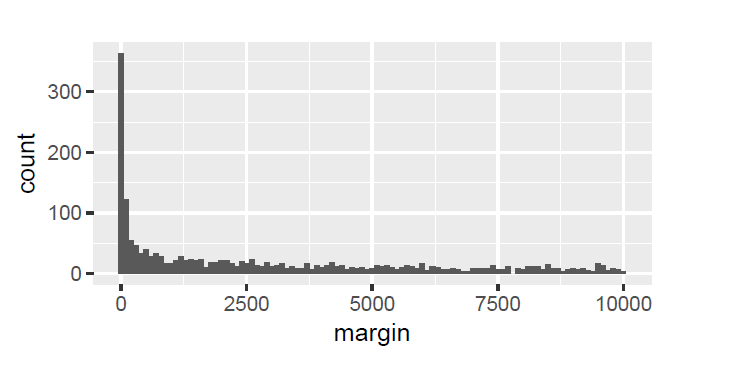
\includegraphics[width=.8\textwidth]{pics/cout_maring.jpg}
    \caption{Customer buying behave}
\end{figure}


Figure 3. Show us that the most customer doesn't spend much money. Also there are no unexpected cluster in the graph.\\


\textbf{Classify the customer}

Because we don't have any clusters in the graph, we separate our customers in four quantiles by the margin. In class one is the customer whos spend lowest money and in class 4 the customers with the most spend money.


$
 Customers < 1.Quantile -> class 1 \\
 1.Quantile < Customers < Median -> class 2 \\
 Median < Customers < 3.Quantile -> class 3 \\
 3.Quantile < Customers -> class 4\\
$

After we had classified, we separated the data in these four classes. 
We filtered the data for only coloured items in order to find out the colour association. For the colour combination rules, we used an apriori algorithm. 
To get the colour combination we checked the most important colour rules and took the mean value of these combinations and plotted it.


% ========================================================
\section{Implementation}



Item frequency: Most bought items.
Now we check the differences in item frequency in these two groups.


\begin{figure}[!htp]        
  \centering
\begin{subfigure}{.63\textwidth}
  \centering
  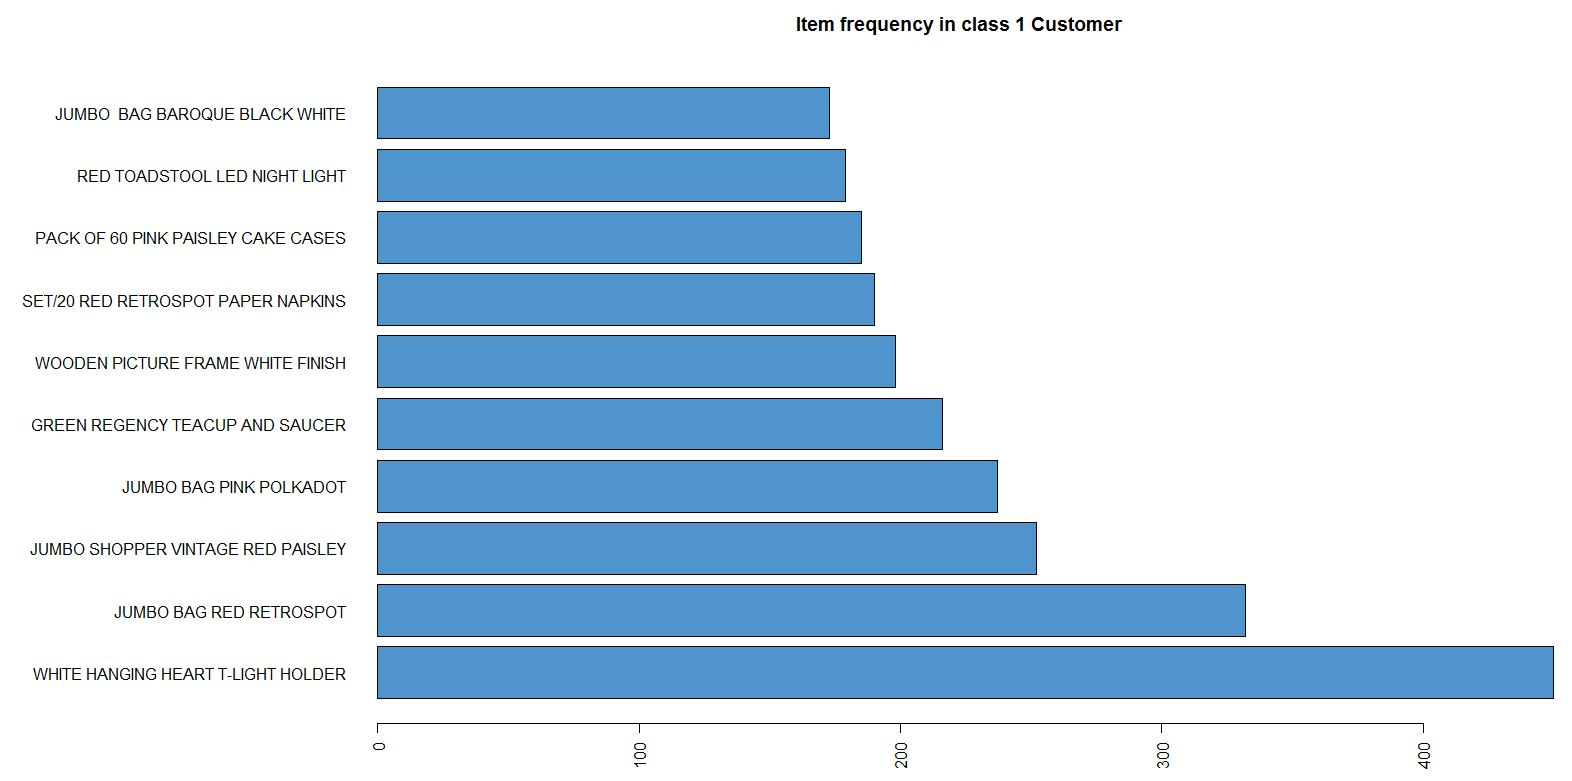
\includegraphics[width=.8\linewidth]{pics/freq1.jpg}
  \caption{Class 1 Customer who spend the lowest quantile}
  \label{fig:sub1}
\end{subfigure}% 
\begin{subfigure}{.63\textwidth}
  \centering
  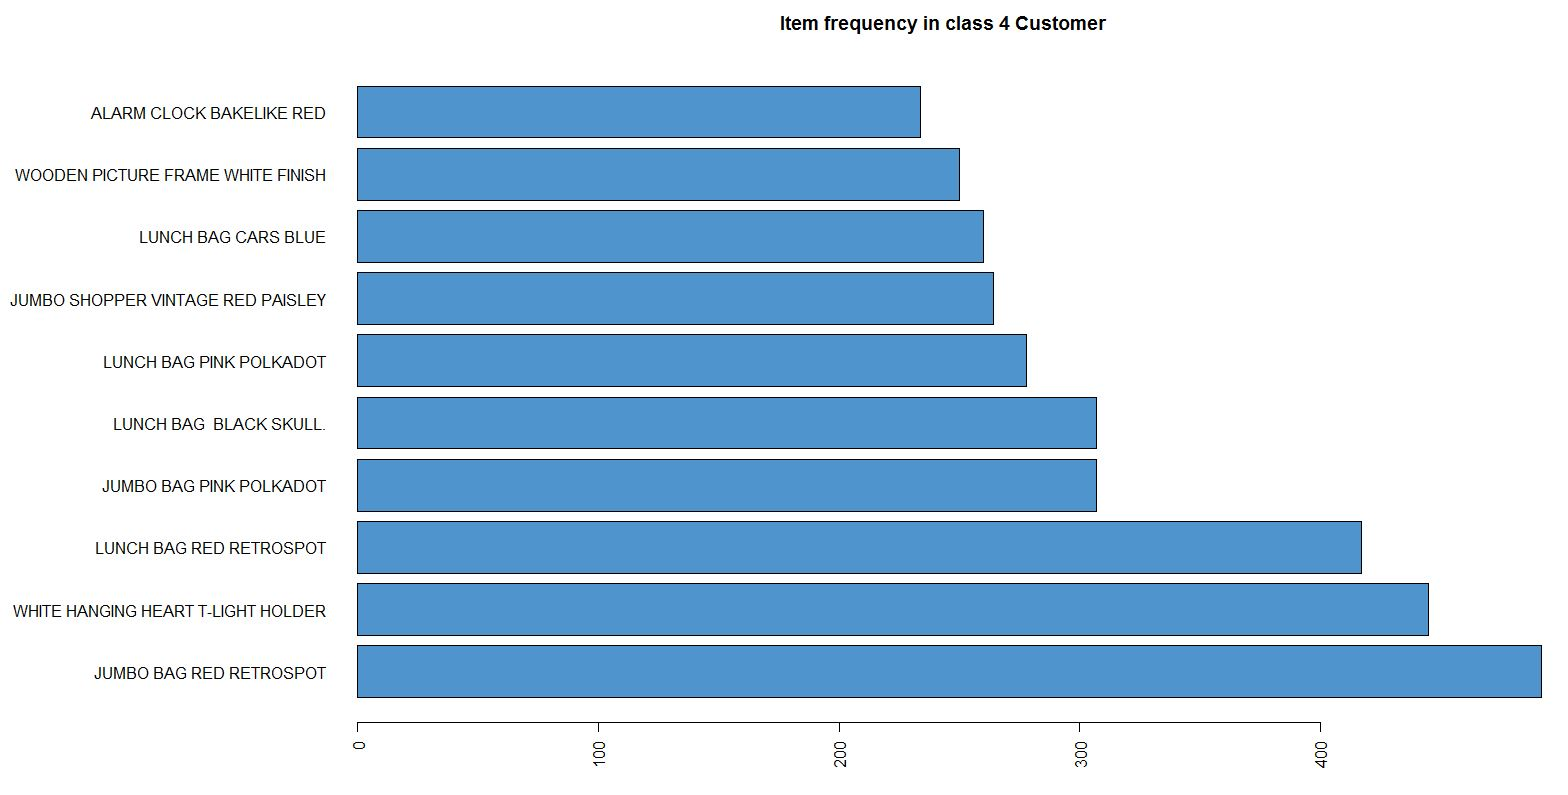
\includegraphics[width=.7\linewidth]{pics/freq4.jpg}
  \caption{Class 4 Customer who spend the highest quantile}
  \label{fig:sub2}
\end{subfigure}
\caption{Differences between two the two classes of customer}
\end{figure}

The Figure 4 shows us that there some are differences in items they bought in these two classes 1 and 4.


\begin{figure}[!htp]        
  \centering
    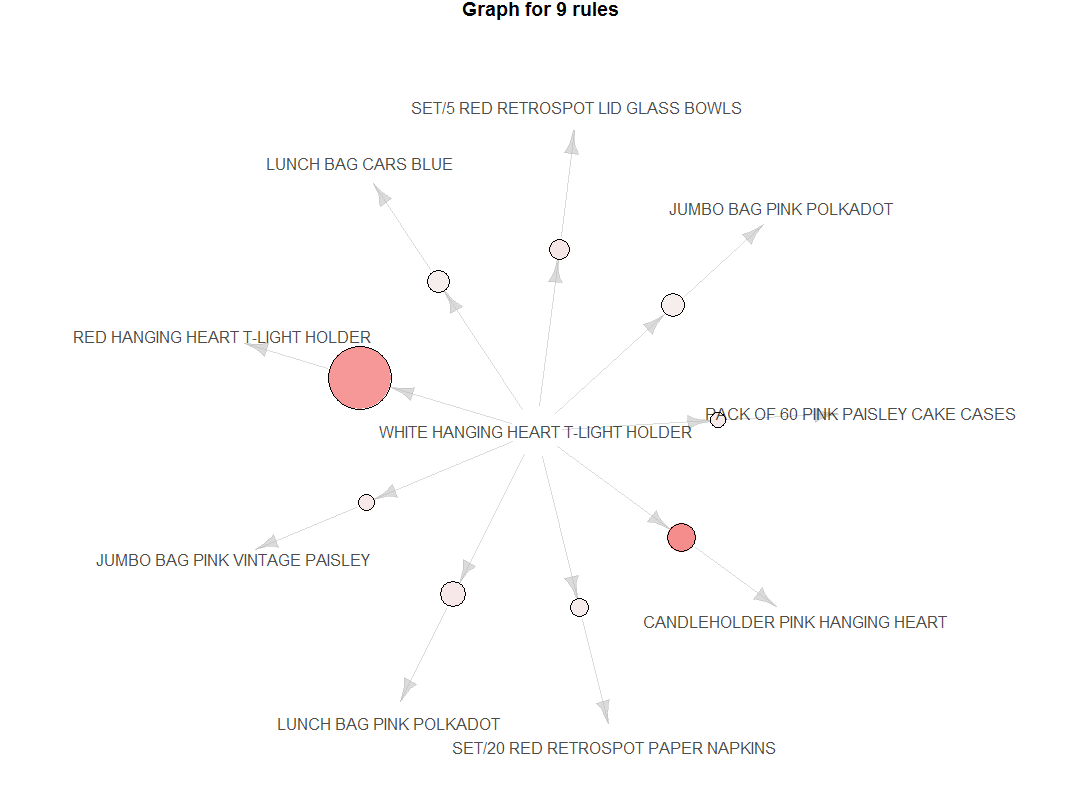
\includegraphics[width=0.5\textwidth]{pics/top9color.jpg}
    \caption{Top 9 Items with other colour that bought with Lighthoulder}
\end{figure}

The Figure 4 and 5 indicates that red and pink items are popular among customers.

Behaviour in Colour associations.

Next we analysed through market basket analyse the strongest connected colors in item sets. 


Top 6 strongest connections in confidence and support.

\begin{figure}[!htp]        
  \centering
    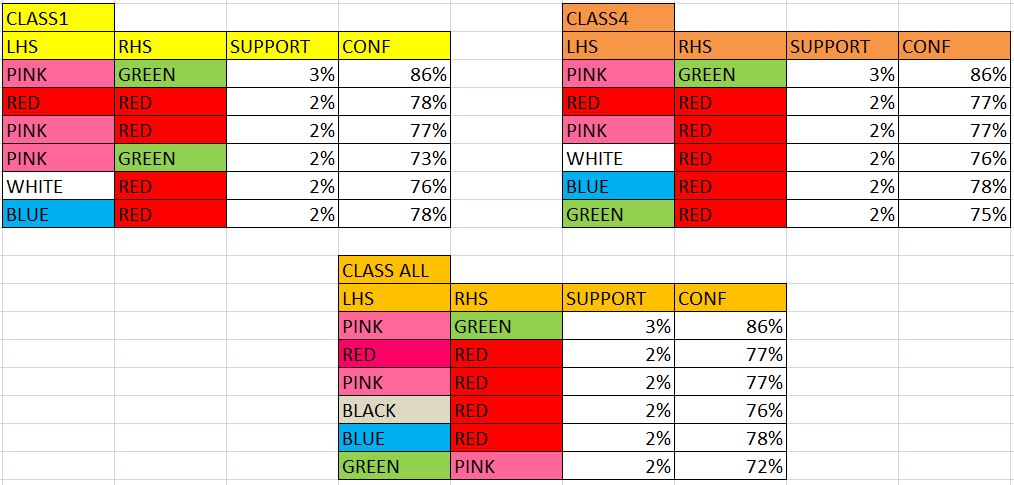
\includegraphics[width=0.7\textwidth]{pics/Combination.jpg}
    \caption{Top 6 Item Color Combination bought by 2 different classes}
\end{figure}
Figure 6 shows us the most preferred colour combinations separated by margin classes and none separated overall colour combination. These tables is arranged by support value from top to bottom. Red and pink items were most preferred and but the green, pink combination is most supported and has most confidence. With these comparisons we see no big differences in these two margin classes.
Because these items are gifts which represent positive feeling means that these colours should be positive associated.
 

\newpage
% ========================================================
\section{Marketing Implications}
This clour combination would save a lot of production cost because we can concentrate it on the most preferenced colour. There are few colours that are preferred more and everybody prefers the same colour even if they buy expansive items. It also helps us to increase the sales in holiday like Christmas.


% ========================================================
\section{Research Implications}
We got positive colour combination that could be sociology, biology and history. 
In Britain the colour red could be seen positive in some context. This could help us to differentiate and classify the colour combination in cultural aspect. 

% ========================================================
\section{Suggestions for future research}
Next task for this project should be making the transform the description in to the category so that we know what category are associated. With a category we can extract more behaviour groups and associate category with colours. The more group we encounter the more individual preferences we get and that could improve the sales and decrease the not sales trashes.
Also, we had to check if the products bought at weekend to clarify if it is bought at home or office environment. Or is it bought on christmas?
Need to differentiate it further. 
And make another dataset that get the behaviour about each Customer so that we can personalise the online webshop and predict their future behaviour. 
For further analysis we need more customer data like gender and age.


% ========================================================

 
\begin{thebibliography}{9}

\bibitem{a}
Randi Priluck Grossman,
\textit{What we know about consumers’ color choices}. 
Seton Hall University, South Orange, New Jersey, USA, 1999
 

\bibitem{b}
Stephen E. Palmera and Karen B. Schlossb,
\textit{Color Preference}. 
Department of Psychology, University of California, Berkeley, Berkeley, CA, USA 2015
 
 
 
 \end{thebibliography}
 
 
\end{document}